\documentclass[../body.tex]{subfiles}
\begin{document}
	
	\subsection{Выборочные коэффициенты корреляции}
	
	\begin{table}[H]
		\centering
		\begin{tabular}{| c | c | c | c |}
			\hline  \hline
			$\rho$ = 0   & $r$    & $r_S$ & $r_Q$ \\ \hline
			$E(z)$       & -0.001 & 0.002 & 0.0   \\ \hline
			$E(z^2)$     & 0.028  & 0.027 & 0.04  \\ \hline
			$D(z)$       & 0.054  & 0.055 & 0.055 \\ \hline
			$\rho$ = 0.5 & $r$    & $r_S$ & $r_Q$ \\ \hline
			$E(z)$       & 0.516  & 0.483 & 0.4   \\ \hline
			$E(z^2)$     & 0.266  & 0.233 & 0.16  \\ \hline
			$D(z)$       & 0.032  & 0.036 & 0.047 \\ \hline
			$\rho$ = 0.9 & $r$    & $r_S$ & $r_Q$ \\ \hline
			$E(z)$       & 0.906  & 0.88  & 0.8   \\ \hline
			$E(z^2)$     & 0.821  & 0.774 & 0.64  \\ \hline
			$D(z)$       & 0.002  & 0.005 & 0.029 \\
			\hline \hline
		\end{tabular}
		\caption{Двумерное нормальное распределение, n = 20}
		\label{tab:n=20}
	\end{table}

	\begin{table}[H]
		\centering
		\begin{tabular}{| c | c | c | c |}
			\hline  \hline
			$\rho$ = 0   & $r$    & $r_S$  & $r_Q$ \\ \hline
			$E(z)$       & -0.008 & -0.005 & 0.0   \\ \hline
			$E(z^2)$     & 0.009  & 0.008  & 0.004 \\ \hline
			$D(z)$       & 0.016  & 0.016  & 0.017 \\ \hline
			$\rho$ = 0.5 & $r$    & $r_S$  & $r_Q$ \\ \hline
			$E(z)$       & 0.502  & 0.481  & 0.333 \\ \hline
			$E(z^2)$     & 0.252  & 0.231  & 0.111 \\ \hline
			$D(z)$       & 0.009  & 0.01   & 0.015 \\ \hline
			$\rho$ = 0.9 & $r$    & $r_S$  & $r_Q$ \\ \hline
			$E(z)$       & 0.902  & 0.888  & 0.733 \\ \hline
			$E(z^2)$     & 0.814  & 0.788  & 0.538 \\ \hline
			$D(z)$       & 0.001  & 0.001  & 0.009 \\
			\hline \hline
		\end{tabular}
	\caption{Двумерное нормальное распределение, n = 60}
	\label{tab:n=60}
	\end{table}

	\begin{table}[H]
		\centering
		\begin{tabular}{| c | c | c | c |}
			\hline \hline
			$\rho$ = 0   & $r$    & $r_S$  & $r_Q$ \\ \hline
			$E(z)$       & -0.006 & -0.008 & 0.0   \\ \hline
			$E(z^2)$     & 0.005  & 0.005  & 0.006 \\ \hline
			$D(z)$       & 0.01   & 0.01   & 0.01  \\ \hline
			$\rho$ = 0.5 & $r$    & $r_S$  & $r_Q$ \\ \hline
			$E(z)$       & 0.499  & 0.479  & 0.32  \\ \hline
			$E(z^2)$     & 0.249  & 0.23   & 0.102 \\ \hline
			$D(z)$       & 0.005  & 0.006  & 0.009 \\ \hline
			$\rho$ = 0.9 & $r$    & $r_S$  & $r_Q$ \\ \hline
			$E(z)$       & 0.902  & 0.89   & 0.72  \\ \hline
			$E(z^2)$     & 0.813  & 0.791  & 0.518 \\ \hline
			$D(z)$       & 0.0    & 0.001  & 0.005 \\
			\hline \hline
		\end{tabular}
		\caption{Двумерное нормальное распределение, n = 100}
		\label{tab:n=100}
	\end{table}

	\begin{table}[H]
		\centering
		\begin{tabular}{| c | c | c | c |}
			\hline  \hline
			$n = 20$  & $r$   & $r_S$ & $r_Q$ \\ \hline
			$E(z)$    & 0.804 & 0.773 & 0.6   \\ \hline
			$E(z^2)$  & 0.647 & 0.597 & 0.36  \\ \hline
			$D(z)$    & 0.032 & 0.012 & 0.008  \\ \hline
			&&&\\ \hline
			$n = 60$  & $r$   & $r_S$ & $r_Q$ \\ \hline
			$E(z)$    & 0.794 & 0.771 & 0.6   \\ \hline
			$E(z^2)$  & 0.63  & 0.595 & 0.36  \\ \hline
			$D(z)$    & 0.012 & 0.004 & 0.003 \\ \hline
			&&&\\ \hline
			$n = 100$ & $r$   & $r_S$ & $r_Q$ \\ \hline
			$E(z)$    & 0.794 & 0.775 & 0.56  \\ \hline
			$E(z^2)$  & 0.63  & 0.6   & 0.314 \\ \hline
			$D(z)$    & 0.007 & 0.002 & 0.001  \\
			\hline  \hline
		\end{tabular}
		\caption{Смесь нормальных распределений}
		\label{tab:mixed}
	\end{table}

	\subsection{Эллипсы рассеивания}
	
	\begin{figure}[H]
		\centering
		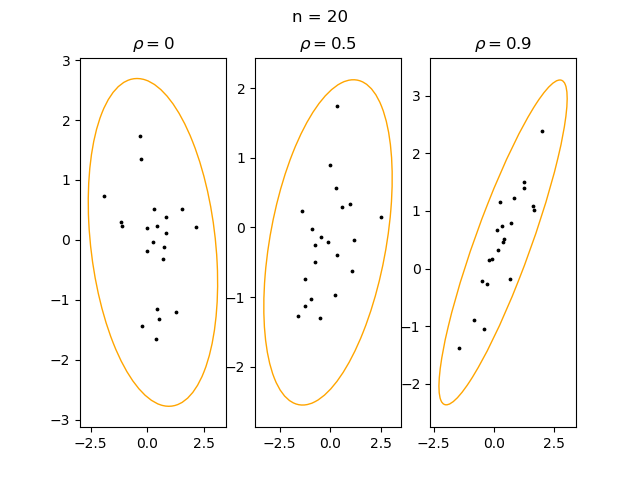
\includegraphics[width = 12cm, height = 8cm]{img/Ellipse n = 20.png}
		\caption{ Двумерное нормальное распределение, n = 20}
		\label{fig:f20}
	\end{figure}
	
	\begin{figure}[H]
		\centering
		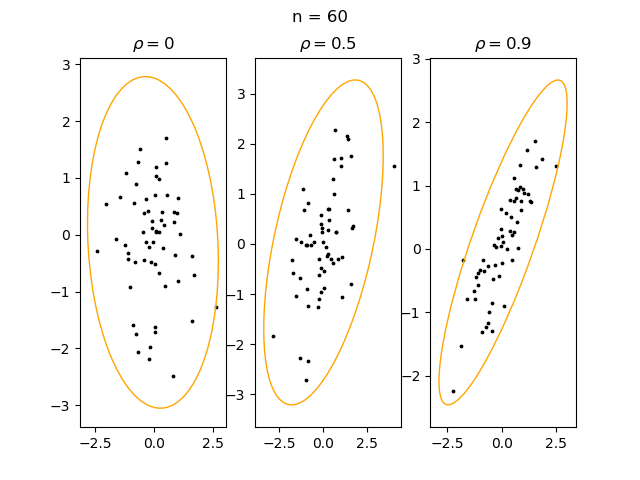
\includegraphics[width = 12cm, height = 8cm]{img/Ellipse n = 60.png}
		\caption{Двумерное нормальное распределение, n = 60}
		\label{fig:f60}
	\end{figure}
	
	\begin{figure}[H]
		\centering
		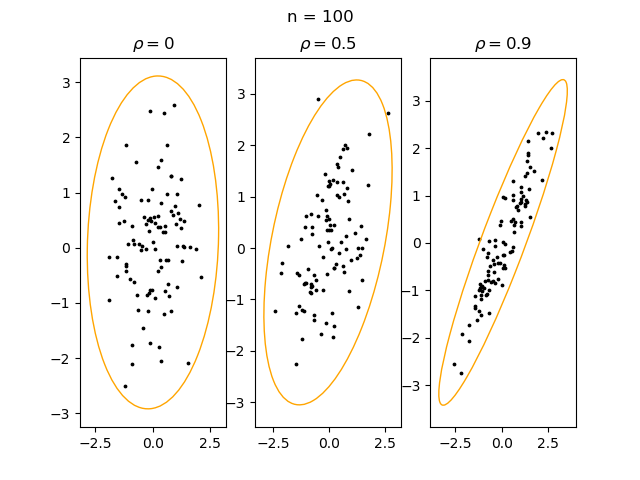
\includegraphics[width = 12cm, height = 8cm]{img/Ellipse n = 100.png}
		\caption{Двумерное нормальное распределение, n = 100}
		\label{fig:f100}
	\end{figure}
	

\end{document}